% !TEX TS-program = xelatex
% !TEX encoding = UTF-8

\documentclass[11pt]{article} 
\usepackage[top=0pt,left=1.5cm,right=1.5cm,bottom=1.5cm,showframe=flse]{geometry}
\usepackage{fontspec} 
\defaultfontfeatures{Mapping=tex-text} 
\usepackage{xunicode} 
\usepackage{xltxtra} 
\usepackage{geometry}
\usepackage{xcolor}
\usepackage{graphicx} 
\makeatletter
\newif\if@debug
\@debugfalse
\if@debug\def\rulecolor{gray}\else\def\rulecolor{white}\fboxsep0pt \fboxrule0pt\fi
\makeatother
\begin{document}

\scalebox{0.5}{\vbox{\hbox{{\color{\rulecolor}\rule{2cm}{3cm}} \fbox{
\includegraphics{img-01}}}

\hbox{{\color{\rulecolor}\rule{3.8cm}{1pt}} \fbox{
\includegraphics{img-02}}\hskip0.8cm \raise7cm\vbox{\fbox{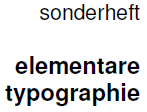
\includegraphics{img-03}}}}

\vspace*{-5cm}\vbox to 0cm{\hbox to 0pt{\hskip 11cm\fbox{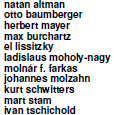
\includegraphics{img-04}}}}

\vspace*{-11.7cm}\vbox to 0cm{\hbox to 0pt{\hskip 14.2cm\fbox{
\includegraphics{img-05}}}}
}}

\end{document}
Frank Mittelbach in this answer said: "I would be interested who would attempt to do that in the plain TeX box model approach. Here is my approach which I will from now onwards call it for simplicity, the pauper's coffins approach". 

If one removes all the `fbox`, the `scalebox ` and the first `vbox` that is used in order to make the `scalebox` work, properly. I am also sure that the code can be reduced to a one line statement and here is my question: Can you produce this layout with a one line statement?.

http://tex.stackexchange.com/a/44159/963




